  % this file is called up by thesis.tex
% content in this file will be fed into the main document
% ----------------------- name of chapter  -------------------------
%\newgeometry{top=-0.4cm, left=0.9cm, right=1.5cm}
\chapter{Kinematic distributions in the Control Regions}
\label{app:CRs}
% ----------------------- paths to graphics ------------------------

% change according to folder and file names
\ifpdf
\graphicspath{Appendices/AP5/figures/}
\else
\graphicspath{Appendices/AP5/figures/}
\fi
\vspace{-0.5cm}
This appendix shows some kinematic distributions in the Control Regions:
\begin{itemize}
	\item \ttbar CR (\Cref{app:CRs:tt});
	\item \ttZ CR (\Cref{app:CRs:ttZ});
	\item Side-band CR1 (\Cref{app:CRs:SB1});
	\item Side-band CR2 (\Cref{app:CRs:SB2});
\end{itemize}

\newpage
\section{\ttbar CR}
\label{app:CRs:tt}
%
%-------------------------------------------------------------------------------
\Cref{fig:sel:cr:ttbar:leps,fig:sel:cr:ttbar:jets} show the distributions 
of kinematic variables for events selected in the \ttbar CR region.

\begin{figure}[!htbp]
	\centering
	\begin{tabular}{cc}
		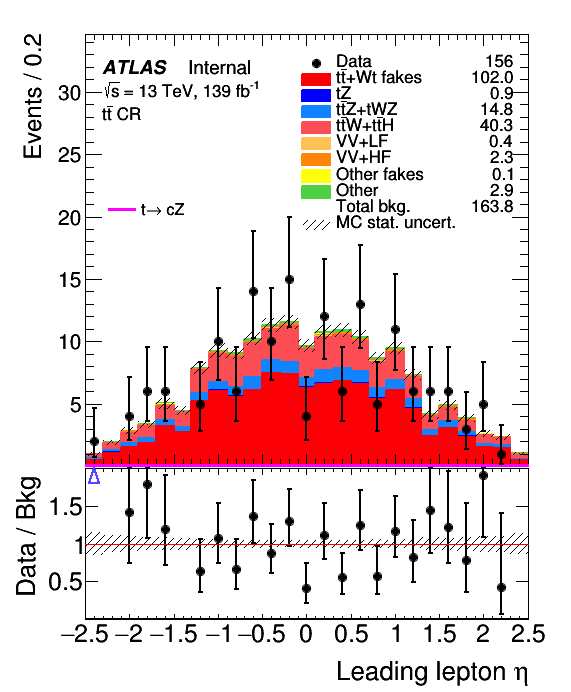
\includegraphics[width=.32\textwidth]{Appendices/AP5/figures/TTCR/lep1_eta} &
		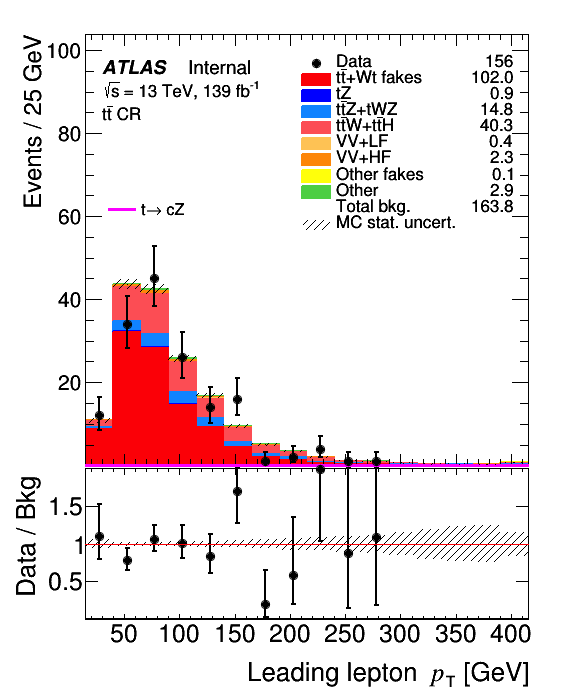
\includegraphics[width=.32\textwidth]{Appendices/AP5/figures/TTCR/lep1_pt} \\
		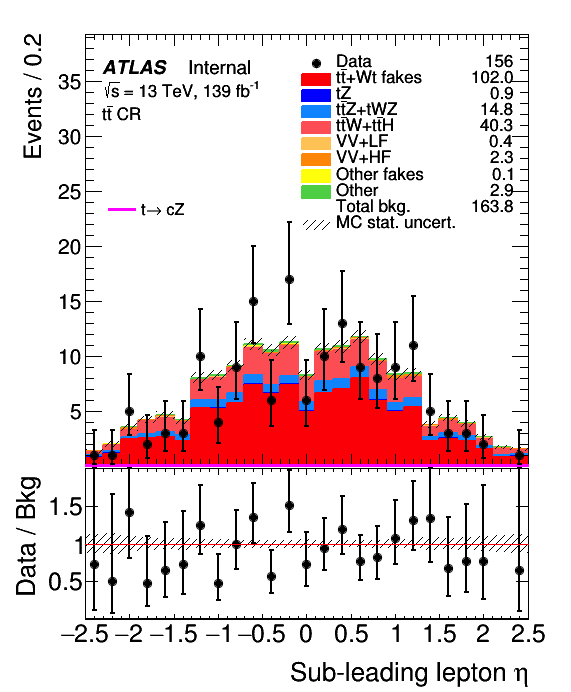
\includegraphics[width=.32\textwidth]{Appendices/AP5/figures/TTCR/lep2_eta} &
		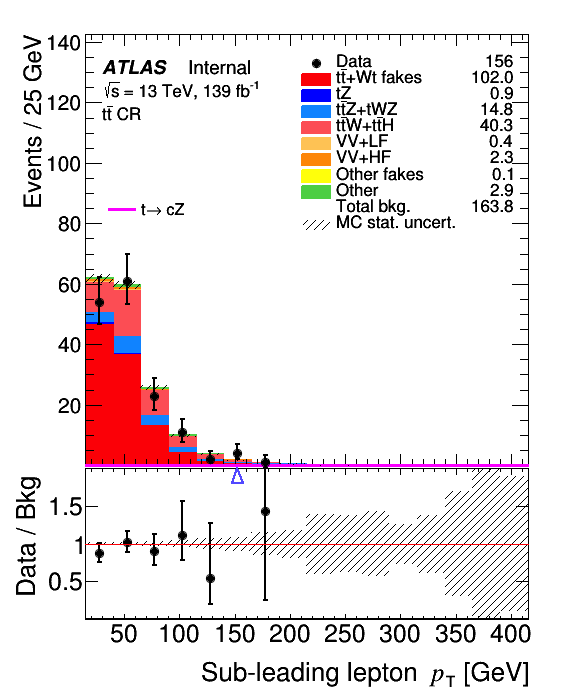
\includegraphics[width=.32\textwidth]{Appendices/AP5/figures/TTCR/lep2_pt} \\
		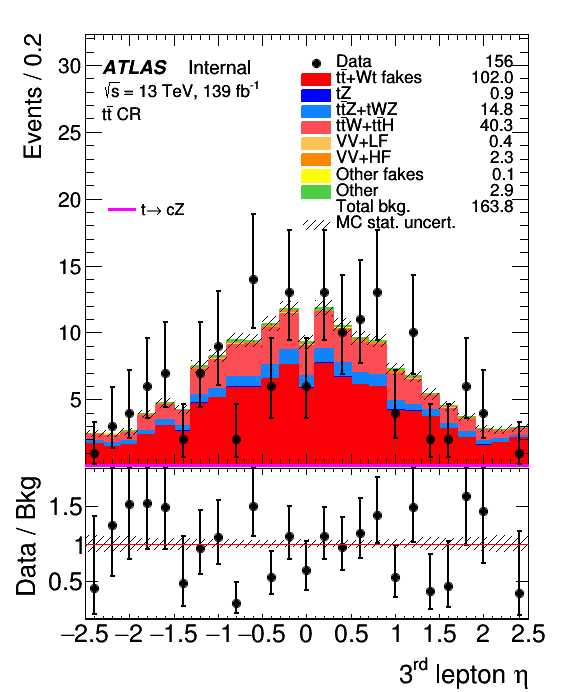
\includegraphics[width=.32\textwidth]{Appendices/AP5/figures/TTCR/lep3_eta} &
		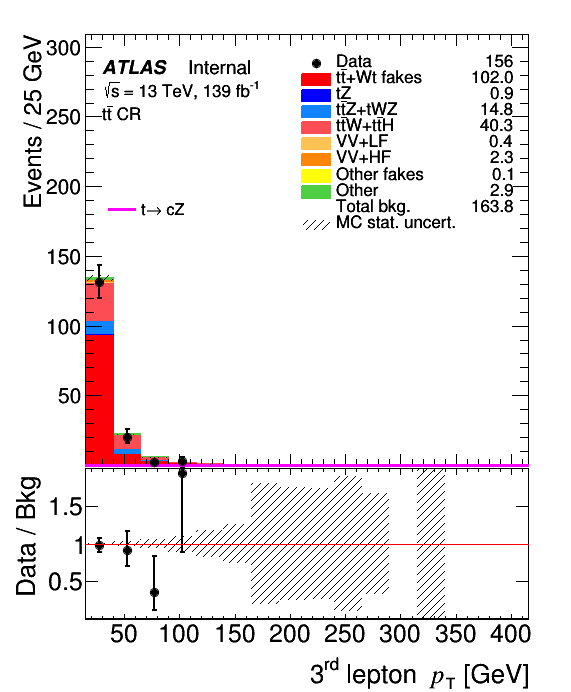
\includegraphics[width=.32\textwidth]{Appendices/AP5/figures/TTCR/lep3_pt} \\
	\end{tabular}
	\caption{Pre-fit distributions of kinematic variables of leptons for events selected in the \ttbar CR.
		\ErrStatOnly
	}%
	\label{fig:sel:cr:ttbar:leps}
\end{figure}

\begin{figure}[]
	\centering
	\begin{tabular}{cc}
		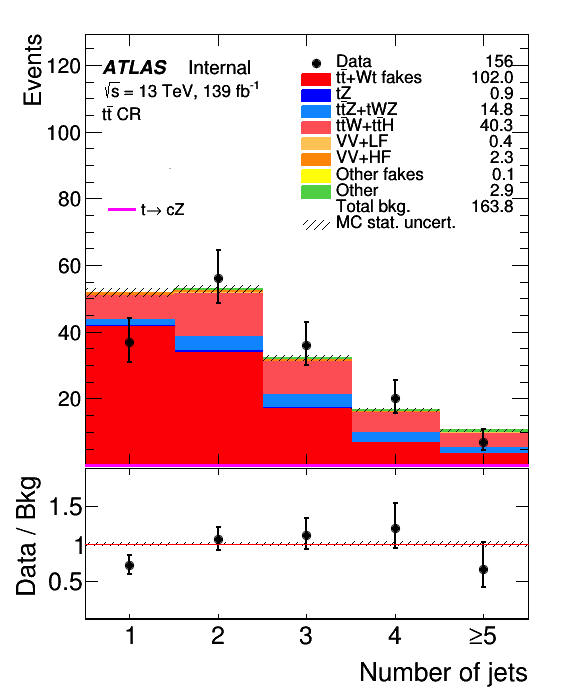
\includegraphics[width=.35\textwidth]{Appendices/AP5/figures/TTCR/nJets} &
		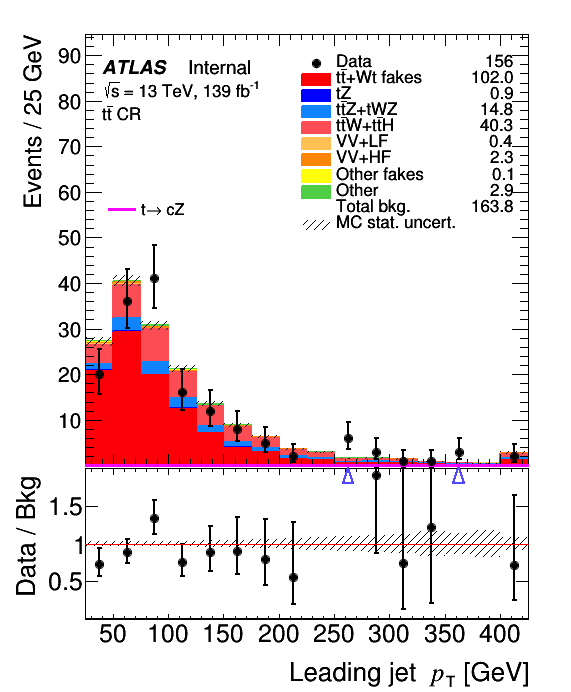
\includegraphics[width=.35\textwidth]{Appendices/AP5/figures/TTCR/jet_pt} \\
		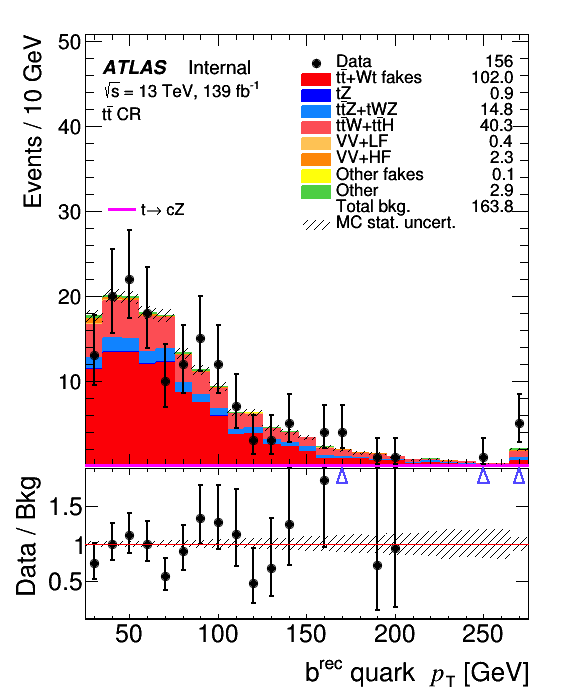
\includegraphics[width=.35\textwidth]{Appendices/AP5/figures/TTCR/b_pt} & 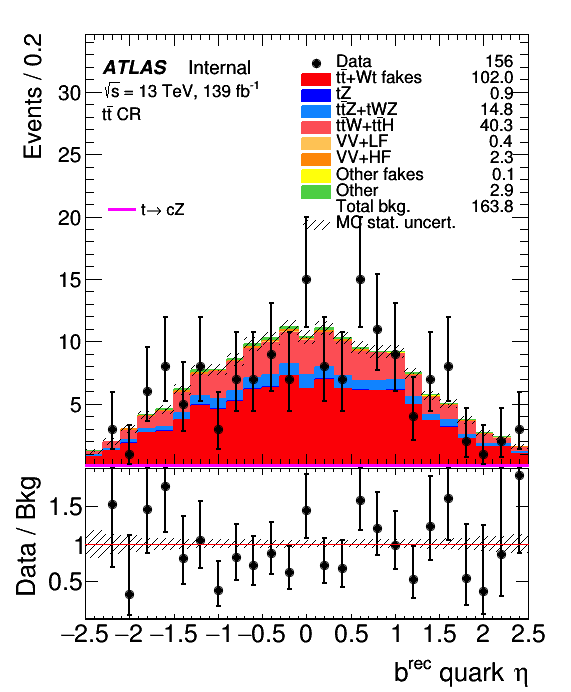
\includegraphics[width=.35\textwidth]{Appendices/AP5/figures/TTCR/b_eta} \\
	\end{tabular}
	\caption{Pre-fit distributions of kinematic variables of jets for events selected in the \ttbar CR.
		\ErrStatOnly
	}%
	\label{fig:sel:cr:ttbar:jets}
\end{figure}

\clearpage
\FloatBarrier
% -------------------------------------------------------------------------------
\section{\ttZ CR}
\label{app:CRs:ttZ}
% -------------------------------------------------------------------------------
\Cref{fig:sel:cr:ttz:leps,fig:sel:cr:ttz:jets} show the distributions 
of kinematic variables for events selected in the \ttZ CR region.

\begin{figure}[!htbp]
	\centering
	\begin{tabular}{cc}
		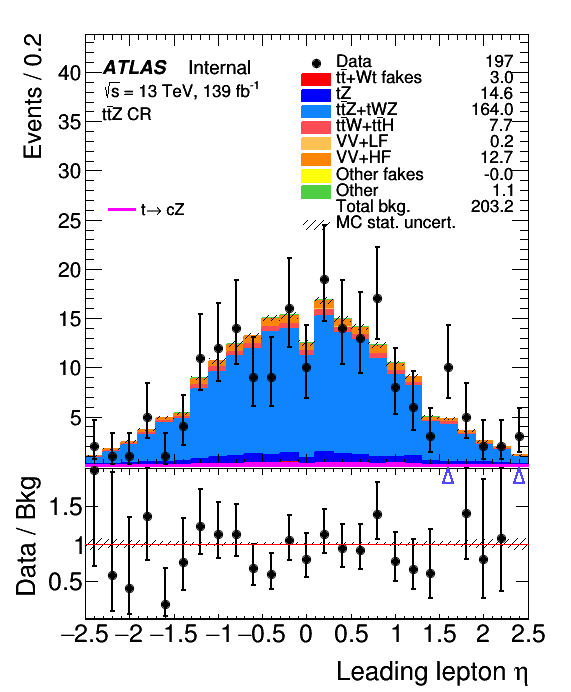
\includegraphics[width=.32\textwidth]{Appendices/AP5/figures/TTZCR/lep1_eta} &
		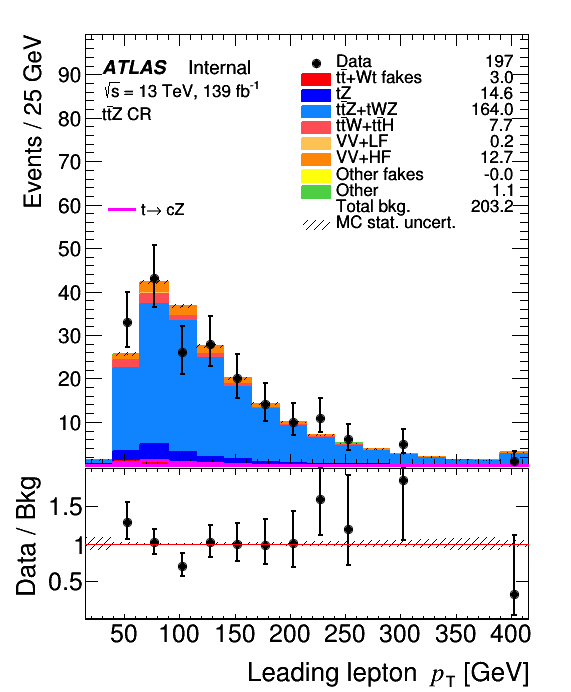
\includegraphics[width=.32\textwidth]{Appendices/AP5/figures/TTZCR/lep1_pt} \\
		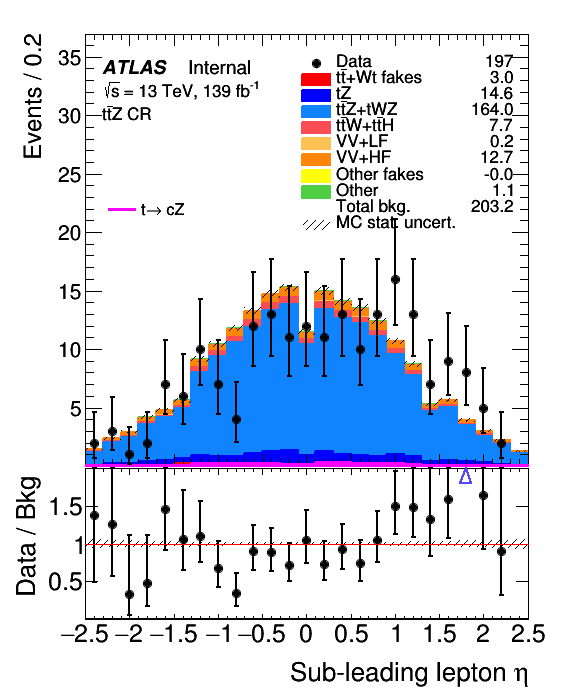
\includegraphics[width=.32\textwidth]{Appendices/AP5/figures/TTZCR/lep2_eta} &
		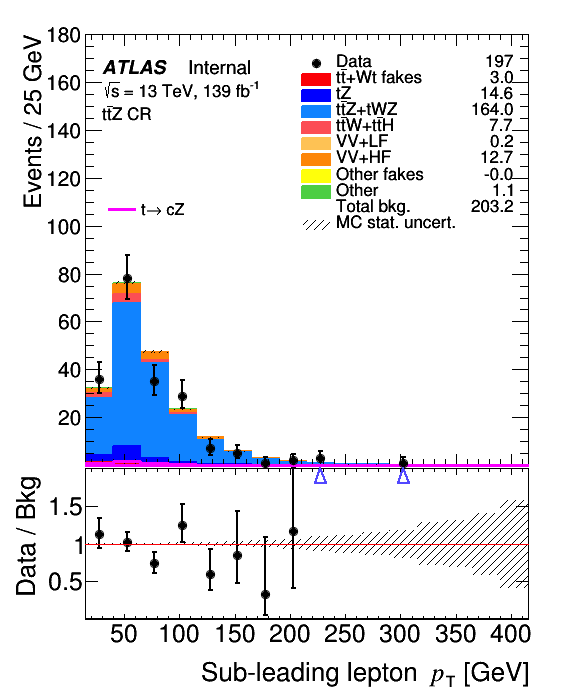
\includegraphics[width=.32\textwidth]{Appendices/AP5/figures/TTZCR/lep2_pt} \\
		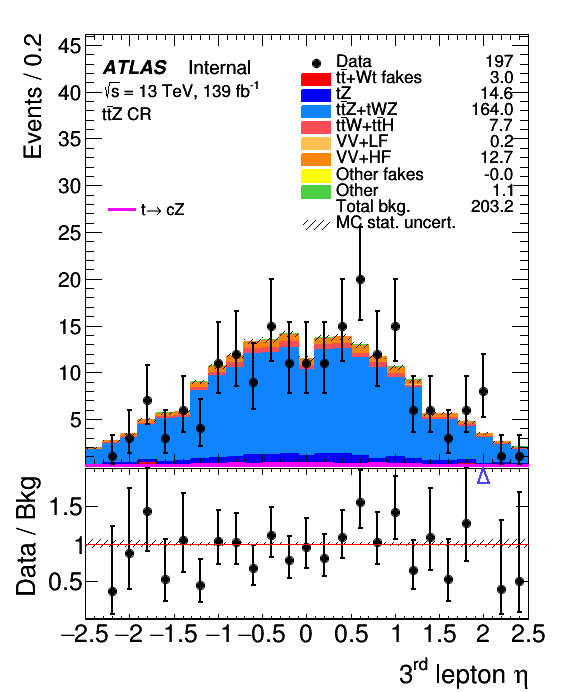
\includegraphics[width=.32\textwidth]{Appendices/AP5/figures/TTZCR/lep3_eta} &
		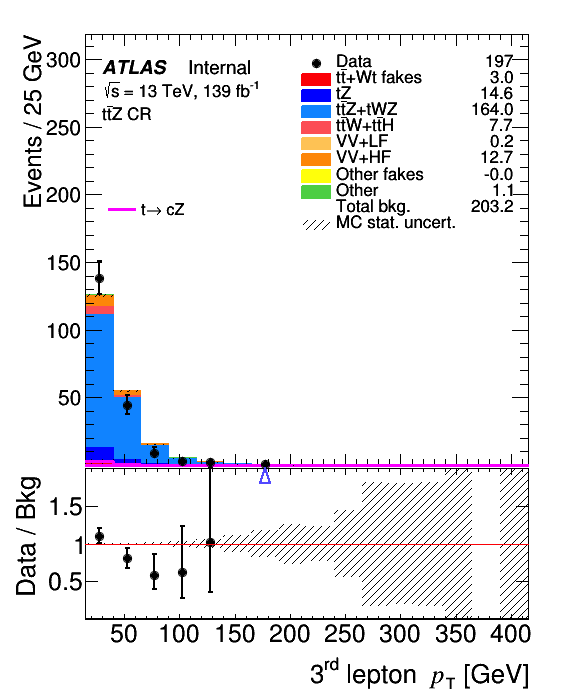
\includegraphics[width=.32\textwidth]{Appendices/AP5/figures/TTZCR/lep3_pt} \\
	\end{tabular}
	\caption{Pre-fit distributions of kinematic variables of leptons for events selected in the \ttZ CR.
		\ErrStatOnly
	}%
	\label{fig:sel:cr:ttz:leps}
\end{figure}

\begin{figure}[]
	\centering
	\begin{tabular}{cc}
		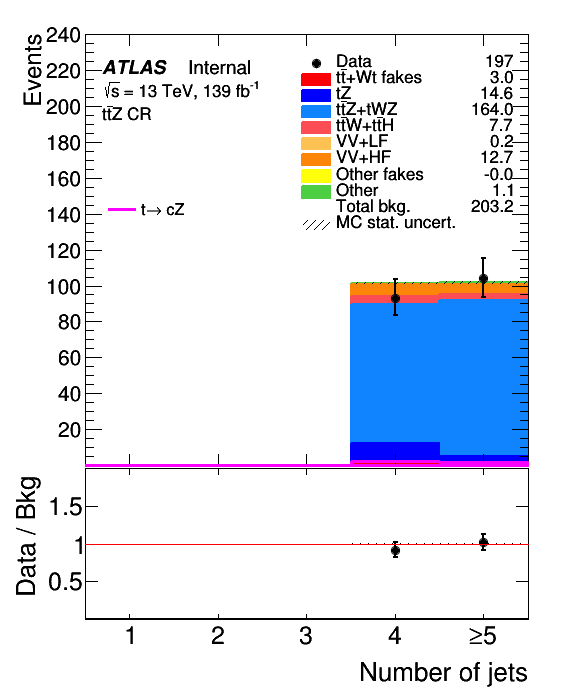
\includegraphics[width=.35\textwidth]{Appendices/AP5/figures/TTZCR/nJets} &
		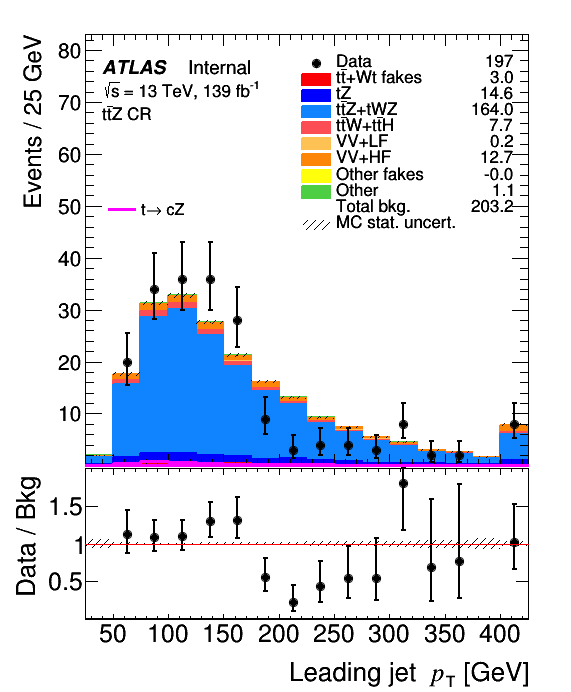
\includegraphics[width=.35\textwidth]{Appendices/AP5/figures/TTZCR/jet_pt} \\
		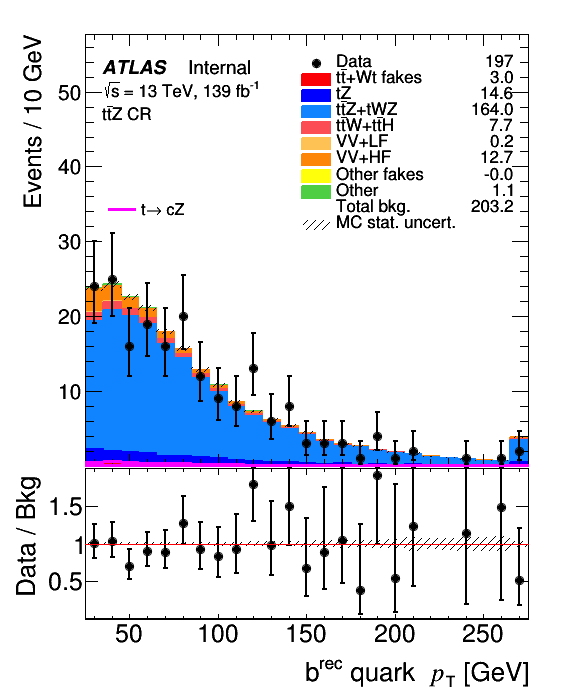
\includegraphics[width=.35\textwidth]{Appendices/AP5/figures/TTZCR/b_pt} &
		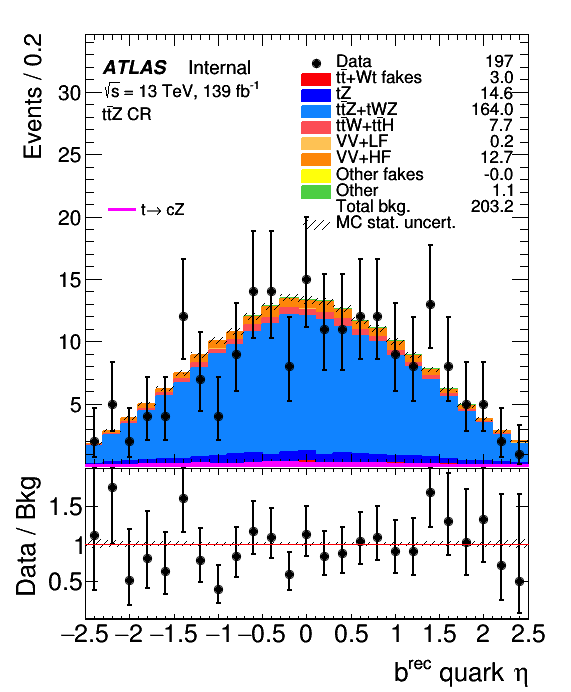
\includegraphics[width=.35\textwidth]{Appendices/AP5/figures/TTZCR/b_eta} \\
	\end{tabular}
	\caption{Pre-fit distributions of kinematic variables of jets for events selected in the \ttZ CR.
		\ErrStatOnly
	}%
	\label{fig:sel:cr:ttz:jets}
\end{figure}

\clearpage
\FloatBarrier
% -----------------------------------------------------------------------------
\section{Side-band CR1}
\label{app:CRs:SB1}
% -------------------------------------------------------------------------------
\Cref{fig:sel:cr:sb1tzc:leps,fig:sel:cr:sb1tzc:jets} show the distributions 
of kinematic variables for events selected in the side-band CR1 region. 

\begin{figure}[!htbp]
	\centering
	\begin{tabular}{cc}
		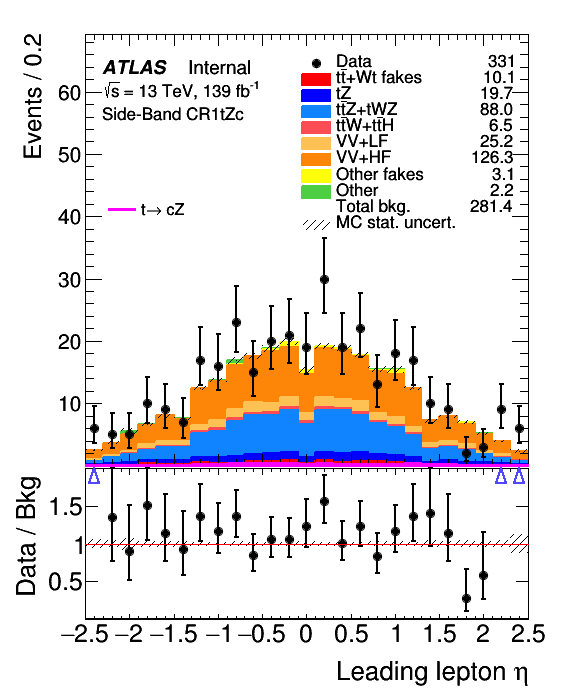
\includegraphics[width=.32\textwidth]{Appendices/AP5/figures/SBCR1/lep1_eta} &
		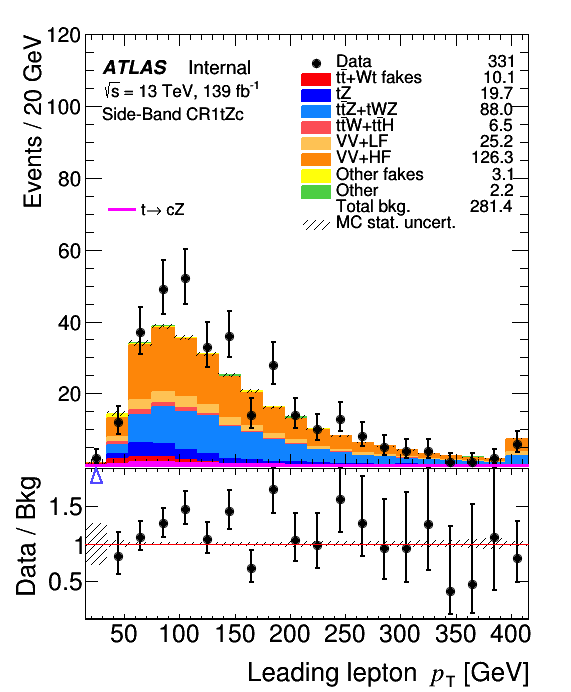
\includegraphics[width=.32\textwidth]{Appendices/AP5/figures/SBCR1/lep1_pt} \\
		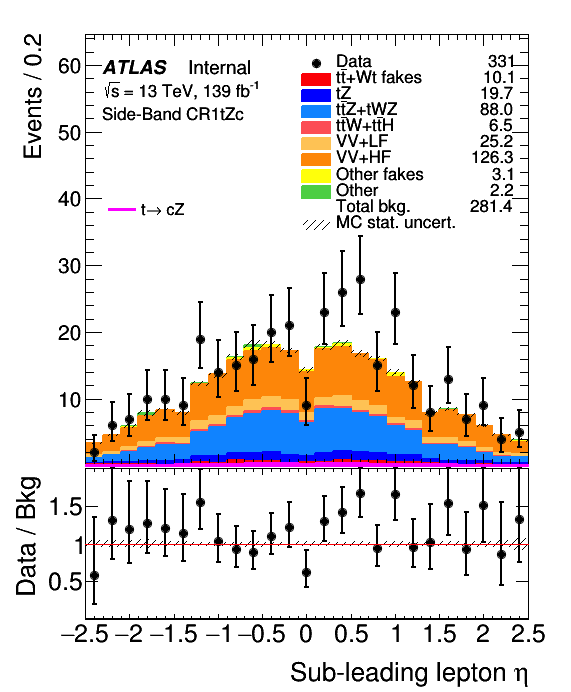
\includegraphics[width=.32\textwidth]{Appendices/AP5/figures/SBCR1/lep2_eta} &
		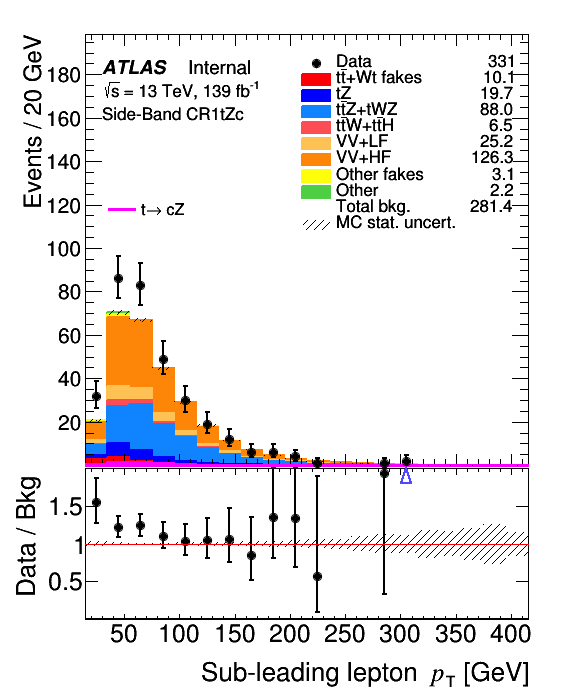
\includegraphics[width=.32\textwidth]{Appendices/AP5/figures/SBCR1/lep2_pt} \\
		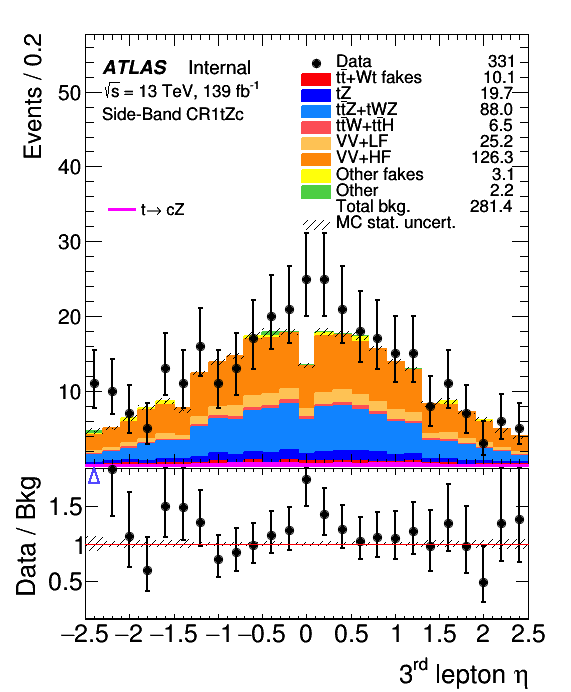
\includegraphics[width=.32\textwidth]{Appendices/AP5/figures/SBCR1/lep3_eta} &
		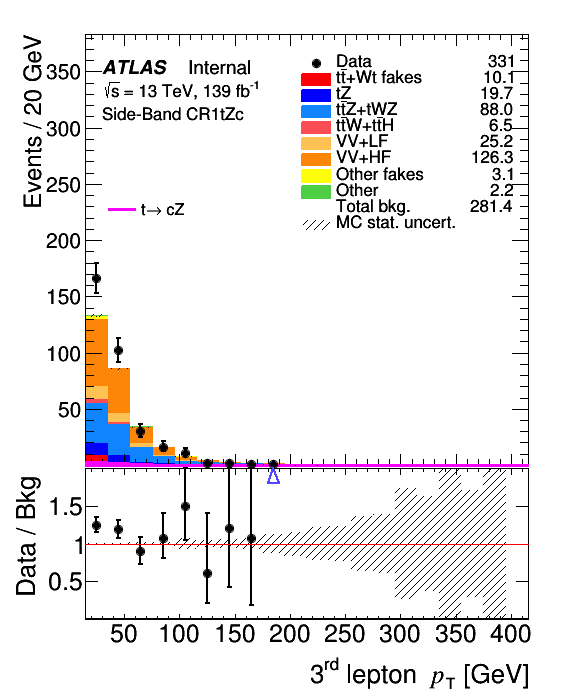
\includegraphics[width=.32\textwidth]{Appendices/AP5/figures/SBCR1/lep3_pt} \\
	\end{tabular}
	\caption{Pre-fit distributions of kinematic variables of leptons for events selected in the side-band CR1 region.
		\ErrStatOnly
	}%
	\label{fig:sel:cr:sb1tzc:leps}
\end{figure}

\begin{figure}[]
	\centering
	\begin{tabular}{cc}
		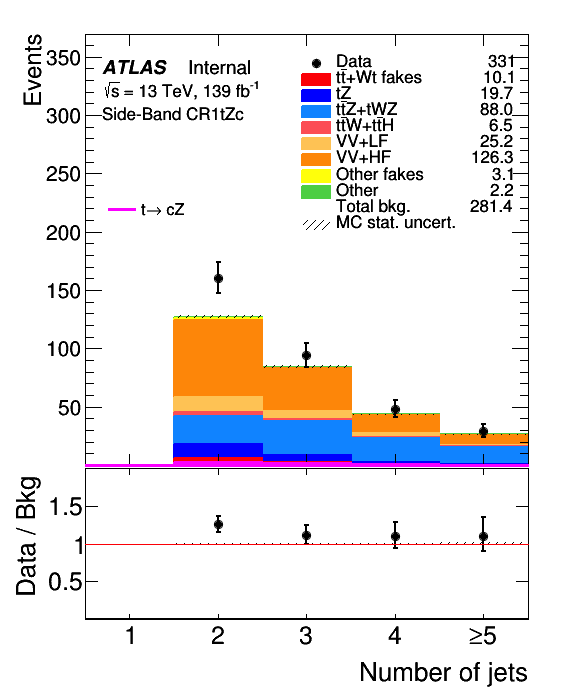
\includegraphics[width=.35\textwidth]{Appendices/AP5/figures/SBCR1/nJets}&
		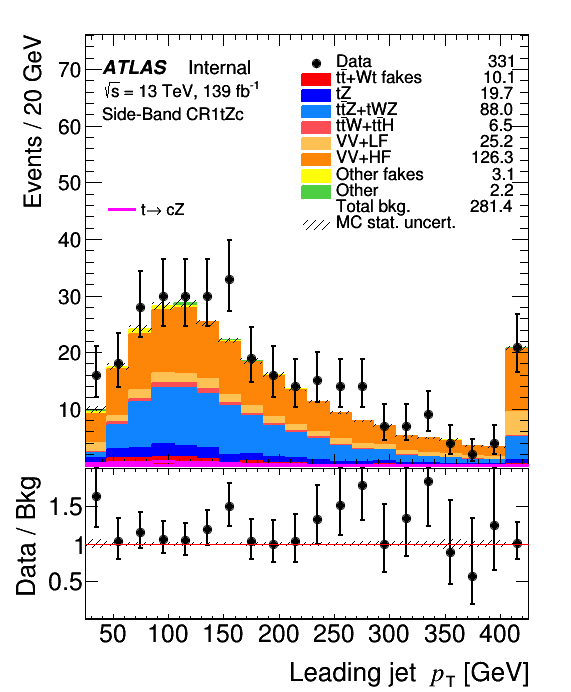
\includegraphics[width=.35\textwidth]{Appendices/AP5/figures/SBCR1/jet_pt} \\
		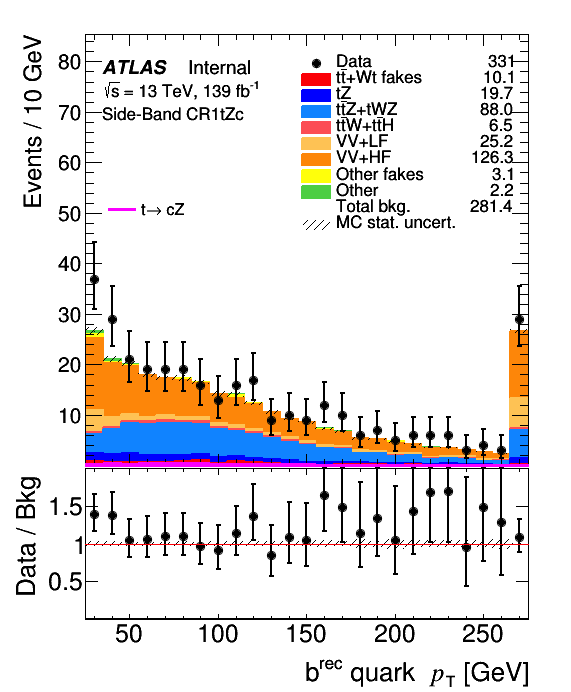
\includegraphics[width=.35\textwidth]{Appendices/AP5/figures/SBCR1/b_pt} &
		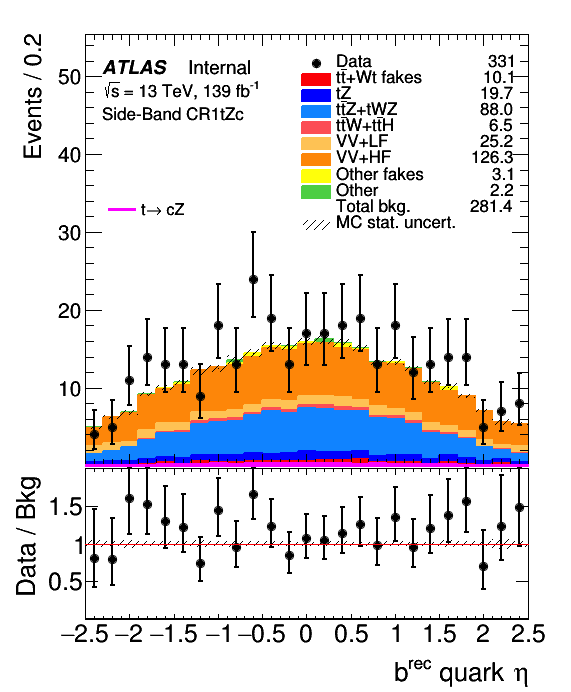
\includegraphics[width=.35\textwidth]{Appendices/AP5/figures/SBCR1/b_eta}\\
	\end{tabular}
	\caption{Pre-fit distributions of kinematic variables of jets for events selected in the side-band CR1 region.
		\ErrStatOnly
	}%
	\label{fig:sel:cr:sb1tzc:jets}
\end{figure}

\clearpage
\FloatBarrier
% -------------------------------------------------------------------------------
\section{Side-band CR2}
\label{app:CRs:SB2}
% -------------------------------------------------------------------------------
\Cref{fig:sel:cr:sb2:leps,fig:sel:cr:sb2:jets} show the distributions 
of kinematic variables for events selected in the side-band CR2 region.

\begin{figure}[!htbp]
	\centering
	\begin{tabular}{cc}
		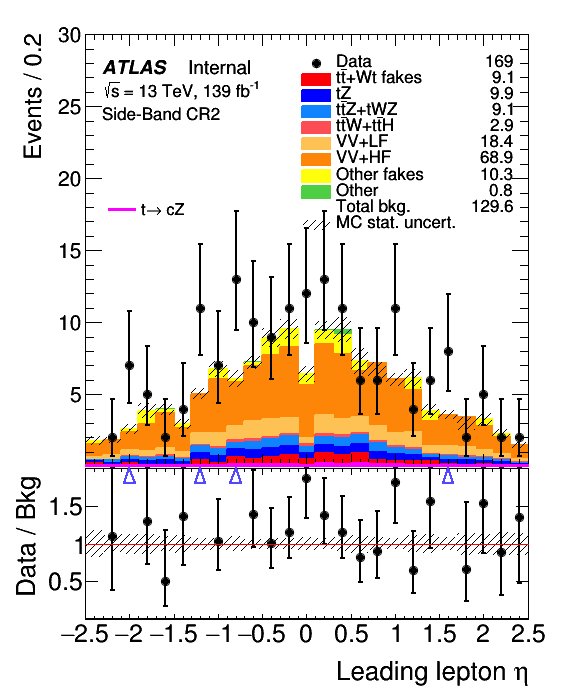
\includegraphics[width=.32\textwidth]{Appendices/AP5/figures/SBCR2/lep1_eta} &
		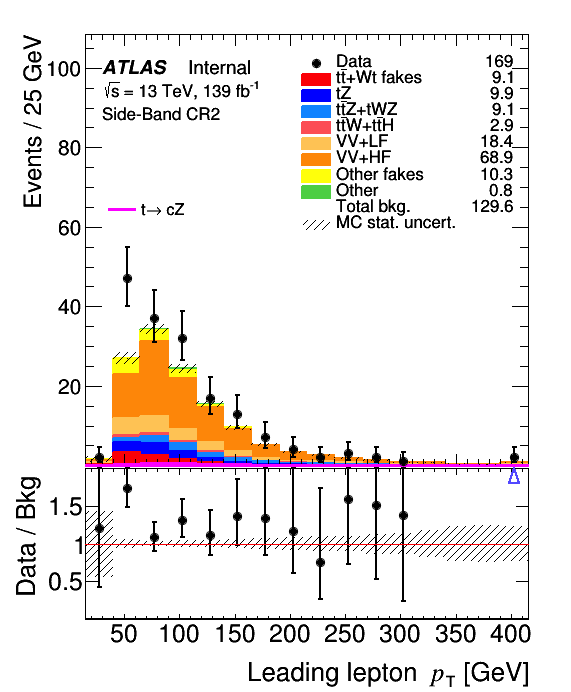
\includegraphics[width=.32\textwidth]{Appendices/AP5/figures/SBCR2/lep1_pt} \\
		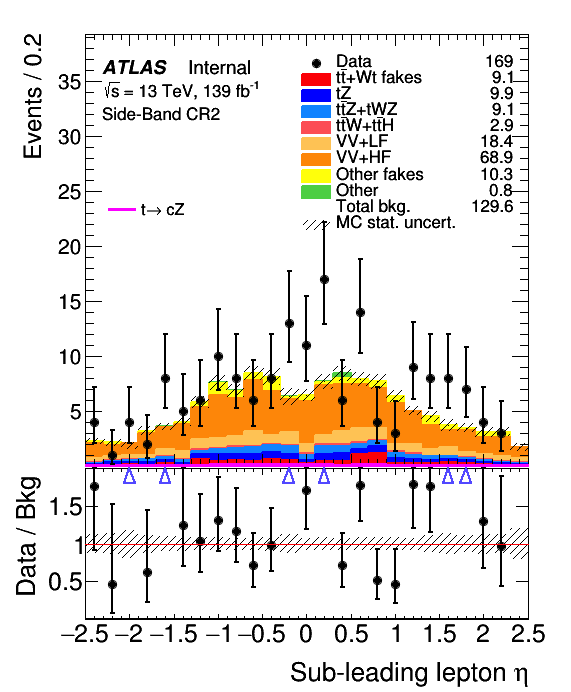
\includegraphics[width=.32\textwidth]{Appendices/AP5/figures/SBCR2/lep2_eta} &
		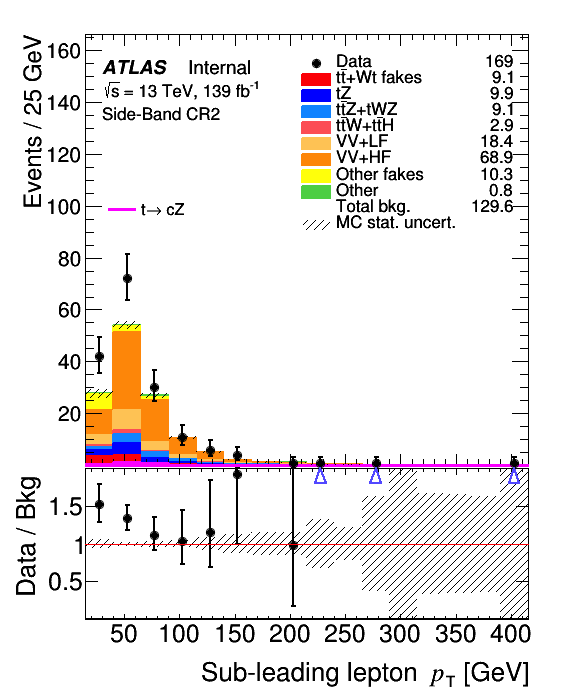
\includegraphics[width=.32\textwidth]{Appendices/AP5/figures/SBCR2/lep2_pt} \\
		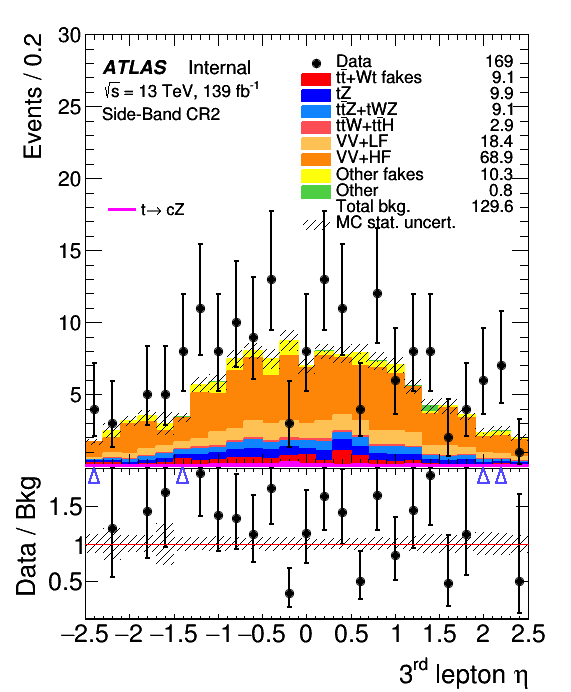
\includegraphics[width=.32\textwidth]{Appendices/AP5/figures/SBCR2/lep3_eta} &
		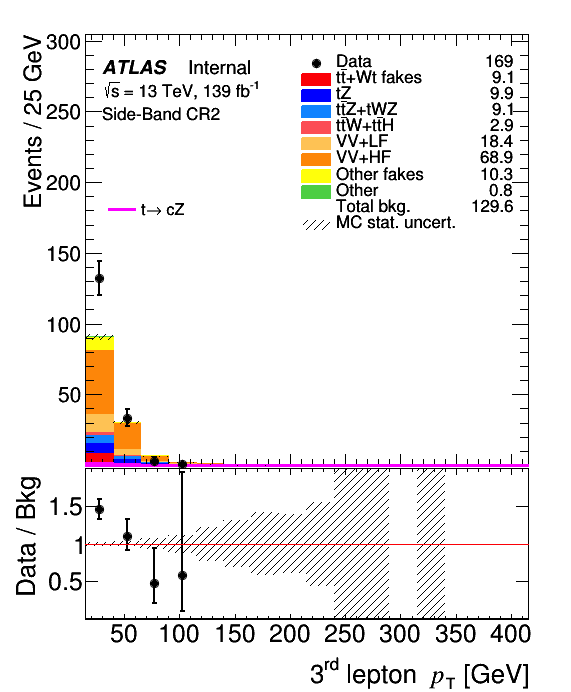
\includegraphics[width=.32\textwidth]{Appendices/AP5/figures/SBCR2/lep3_pt} \\
	\end{tabular}
	\caption{Pre-fit distributions of kinematic variables of leptons for events selected in the side-band CR2 region.
		\ErrStatOnly
	}%
	\label{fig:sel:cr:sb2:leps}
\end{figure}

\begin{figure}[]
	\centering
	\begin{tabular}{cc}
		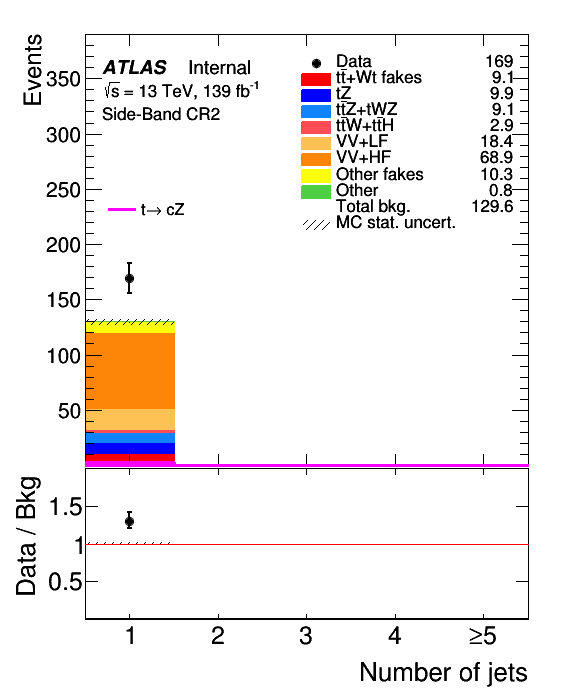
\includegraphics[width=.35\textwidth]{Appendices/AP5/figures/SBCR2/nJets} &
		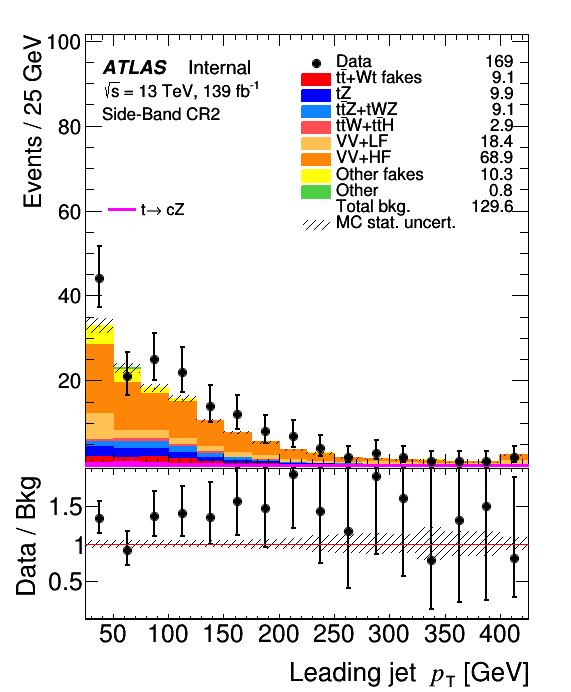
\includegraphics[width=.35\textwidth]{Appendices/AP5/figures/SBCR2/jet_pt} \\
		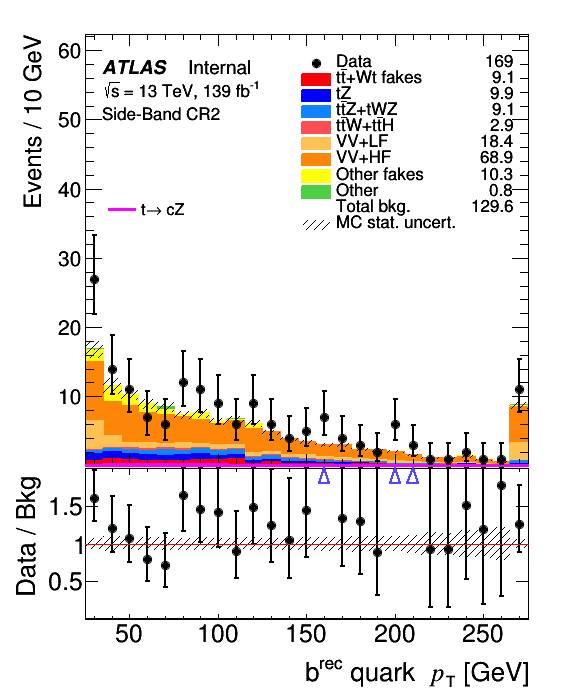
\includegraphics[width=.35\textwidth]{Appendices/AP5/figures/SBCR2/b_pt} &
		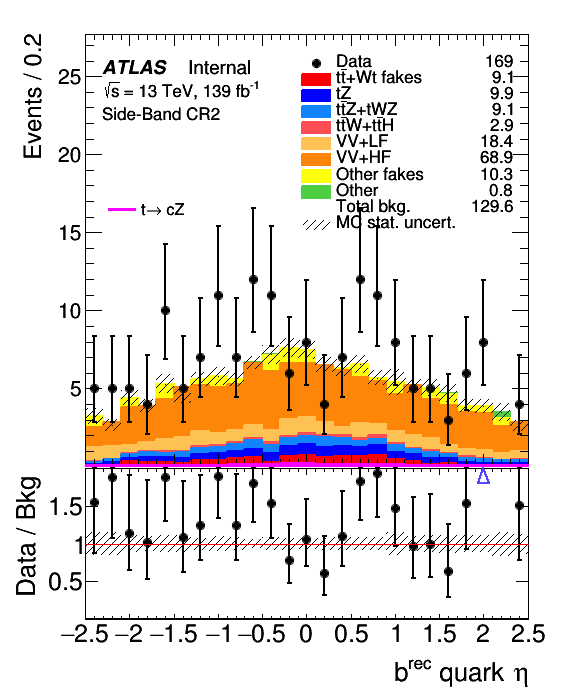
\includegraphics[width=.35\textwidth]{Appendices/AP5/figures/SBCR2/b_eta} \\
	\end{tabular}
	\caption{Pre-fit distributions of kinematic variables of jets for events selected in the side-band CR2 region.
		\ErrStatOnly
	}%
	\label{fig:sel:cr:sb2:jets}
\end{figure}

